\section{Вопросы из билетов}

\subsection{Эквивалентность фундированности, отсутствия бесконечно убывающей последовательности элементов и принципа трансфинитной индукции.}
\noindent Мы будем работать с частично упорядоченным множеством $(A, \leqslant)$ и для краткости будем его просто называть множеством $A$.
\newline \par \textbf{Теорема:} Три определения фундированного множества эквивалентны друг другу:
\begin{enumerate}
    \item Множество $A$ называется фундированным, если в любом непустом подмножестве $A$ есть минимальный элемент.

    \item Множество $A$ называется фундированным, если для него выполняется принцип невозможности бесконечного спуска: не существует бесконечной строго убывающей последовательности $x_1>x_2>x_3>\ldots$
    
    \item Множество $A$ называется фундированным, если для него выполняется принцип трансфинитной индукции: для любого свойства $\phi(x)$ верно условие:
    $$\forall x \; (\forall y<x \;\; \phi(y)\to \phi(x) ) \;\Rightarrow\; \forall x \phi(x).$$
\end{enumerate}

$\blacktriangle$ (1 $\Rightarrow$ 2) Предположим, что 2 определение неверно, и в множестве есть бесконечная убывающая цепь $x_1 > x_2>\ldots$. Но тогда в множестве $B = \{x_1, x_2, \ldots\}$ нет минимального элемента, что противоречит определению 1.

\par 
(2 $\Rightarrow$ 1) Теперь предположим, что определение 1 не выполнено. Это значит, что в $A$ есть непустое подмножество $B$, в котором нет минимального элемента. Поскольку $B\neq \emptyset$, то $\exists x_1\in B$. Мы предположили, что в $B$ нет минимальных элементов. В частности, $x_1\neq min$, то $\exists x_2 < x_1$. Поскольку $x_2\neq min$, то $\exists x_3 < x_2$ и так далее, получим бесконечно убывающую последовательность. Это противоречит определению 2.

\par (1 $\Rightarrow$ 3) Снова предположим, что для
некоторого $A$ выполнено определение 1. Нам нужно доказать, что для данного множества выполнен также и принцип индукции. Пусть для какого-то свойства $\phi(x)$ верен “шаг индукции”: $$\forall x \; (\forall y<x \;\; \phi(y)\to \phi(x) ).$$
Мы хотим показать, что в таком случае свойство $\phi(x)$ верно для всех элементов $x \in A$. Предположим противное – пусть для некоторых $x$ свойство $\phi(x)$ ложно. Выберем среди всех таких $x$ минимальный (определение фундированности гарантирует, что среди всех элементов $x$ для которого $\phi(x)$ ложно, есть хотя бы один минимальный). Тогда для данного $x_{min}$ свойство $\phi(x_{min})$ ложно, а для всех элементов $y$ меньших $x_{min}$ свойство $\phi(y)$ истинно. Получаем противоречие с предположением индукции (т.е. $1\to 0$).

\par (3 $\Rightarrow$ 1) Теперь предполагаем, что для
$A$ выполнен принцип индукции. Нам нужно проверить, что $\forall B\subset A \; | \; B\neq \emptyset$ есть хотя бы один минимальный элемент. Пусть в некотором $B\subset A$ минимального элемента нет. Мы должны доказать, что данное $B$ пусто. Для этого мы рассмотрим свойство $\phi(x)$\;: $\phi(x)$ истинно $\Leftrightarrow \; x\notin B$. Для данного свойства верно: $$\forall x \; (\forall y<x \;\; \phi(y)\to \phi(x) ).$$ 
(если все элементы $y<x$ не лежат в $B$, то и $x$ не лежит в $B$, иначе $x$ был бы минимальным элементом $B$) По принципу индукции заключаем, что свойство $\phi(x)$ истинно для всех $x\in A$. Это значит, что в $B$ нет ни одного
элемента — это подмножество пусто. $\quad \blacksquare$

\subsection{Лемма о монотонной функции из вполне упорядоченного множества в себя.}

\textbf{Лемма:} Пусть $A$ -- вполне упорядоченное множество, а $f:A\to A$ -- строго монотонная функция ($x>y \Rightarrow f(x)>f(y)$). Тогда $\forall x \; f(x)\geqslant x$.

$\blacktriangle$ Докажем через принцип невозможности бесконечного спуска:
\newline Пусть для какого-то $x$ верно $f(x)<x$. Тогда по строгой монотонности выполнено: $$f(f(x))<f(x),\;\; f(f(f(x)))<f(f(x)),\;\; \ldots$$ Следовательно, образуется бесконечно убывающая последовательность $$x>f(x)>f(f(x))>f(f(f(x)))>\ldots$$ Это противоречит фундированности $A$, значит, $\forall x \; f(x)\geqslant x$. $\quad \blacksquare$

\subsection{Теорема о структуре вполне упорядоченного множество: оно представляется как $\omega \cdot L + F$, где $L$ — множество предельных элементов (кроме, возможно, наибольшего), $F$ — конечное множество.}

\par $\blacktriangle$ Пусть $P$ -- множество предельных элементов нашего ВУМа. Заметим, что $P$ -- ВУМ (как подмножество ВУМа). Рассмотрим элемент $x \in P$. Пусть $Sx=y$ (следующий элемент). Построим биекцию между $\omega$ и $[x, y)$. Числу $n$ из $\omega$ поставим в соответствие число $\underbrace{SS\ldots S}_\text{$n$ раз}x$. Очевидно, что это инъекция ($x+n=x+m \Leftrightarrow n=m$).
\par Докажем, что это сюръекция. Рассмотрим элемент $t$ лежащий в $[x,y)$. Бесконечно уменьшать его на 1 (то есть брать предыдущий) нельзя по одному из эквивалентных определений фундированности $\Rightarrow$ существует предельный элемент $k$ (у которого нет предыдущего), такой что  $S\ldots Sk=t$. $k$ лежит в $[x,y)$, но единственный предельный элемент, лежащий в этом множестве -- это $x \Rightarrow k=x \Rightarrow t=S\ldots Sk$ будет получен. 
\par Повторим такие действия для всех $x$ (кроме наибольшего). Затем возможны 2 случая
\begin{enumerate}
    \item В исходном ВУМе нет наибольшего элемента. Тогда аналогично прошлым шагам строим изоморфизм между $\omega$ и оставшимися элементами. Получаем, что наш ВУМ равен $\omega \cdot P$.
    \item В исходном ВУМе есть наибольший элемент. Тогда осталось лишь конечное число нерассмотренных элементов. Докажем это.
    \par Обозначим наибольший элемент всего ВУМа как $a$. По определению фундированности, мы не сможем бесконечно брать предыдущий элемент $\Rightarrow$ существует $k$ -- предельный, такой что $a=\underbrace{S\ldots S}_\text{$m$ раз}k$. $k \geq x,$ но $x$ -- наибольший из предельных элементов $\Rightarrow$ $k=x \Rightarrow |[x;a]|=m+1$. Построим биекцию между этим отрезком и множеством $F=[0;m]$.
\end{enumerate}

\par Таким образом, получаем, что наше ВУМ равномощно $\omega \cdot L + F$, где $L$ -- множество предельных элементов кроме, возможно, наибольшего, а $F$ -- конечное множество. $\blacksquare$

\subsection{Теорема о трансфинитной рекурсии.}

\textbf{Теорема.} Пусть $A$ -- вполне упорядоченное множество, $B$ -- произвольное множество. Пусть имеется некоторое рекурсивное правило (отображение $F$, которое ставит в соответствие элементу $x \in A$ и функции $g : [0, x) \rightarrow B$ некоторый элемент $B$). Тогда $\exists !$ функция $f : A \rightarrow B$: $f(x) = F(x, f|_{[0,x)})$ $\forall x \in A$. (здесь $f|_{[0,x)}$ обозначает ограничение функции $f$ на начальный отрезок $[0, x)$)

$\blacktriangle$
Идея доказательства: значение $f$ на минимальном элементе определено однозначно, так как предыдущих значений нет (сужение $f|_{[0,0)}$ пусто). Тогда и на следующем элементе значение функции $f$ определено однозначно, поскольку на предыдущих (точнее, единственном предыдущем) функция $f$ уже задана, и т. д.

Строгое док-во:

1. Утверждение о произвольном $a \in A$: существует и единственно отображение $f$ отрезка $[0, a]$ в множество $B$, для которого рекурсивное определение (равенство, приведённое в условии) выполнено при всех $x \in [0, a]$.

Пусть отображение $f : [0, a] \rightarrow B$, обладающее указанным свойством -- "корректное". Таким образом, мы хотим доказать, что $\forall a \in A$ $\exists!$ корректное отображение отрезка $[0, a]$ в $B$. Поскольку мы рассуждаем по индукции, можно предполагать, что для всех $c < a$ это утверждение выполнено, то есть существует и единственно корректное отображение $f_c : [0, c] \rightarrow B$. (Корректность $f_c$ означает, что при всех $d \leqslant c$ значение $f_c(d)$ совпадает с предписанным по рекурсивному правилу.)

Рассмотрим отображения $f_{c_1}$ и $f_{c_2}$ для двух различных $c_1$ < $c_2$. Отображение $f_{c_2}$ определено на большем отрезке $[0, c_2]$. Если ограничить $f_{c_2}$ на меньший отрезок $[0, c_1]$, то оно совпадёт с $f_{c_1}$, поскольку ограничение корректного отображения на меньший отрезок корректно (это очевидно), а мы предполагали единственность на отрезке $[0, c_1]$.

Таким образом, все отображения $f_c$ согласованы друг с другом (принимают одинаковое значение, если определены одновременно). Объединив их, мы получаем некоторое единое отображение $h$, определённое на $[0, a)$. Применив к $a$ и $h$ рекурсивное правило, получим некоторое значение $b \in B$. Доопределим $h$ в точке $a$, положив $h(a) = b$. Получится отображение $h: [0, a] \rightarrow B$; легко понять, что оно корректно.

Чтобы завершить индуктивный переход, надо проверить, что на отрезке $[0, a]$ корректное отображение единственно. В самом деле, его ограничения на отрезки $[0, c]$ при $c < a$ должны совпадать с $f_c$, поэтому осталось проверить однозначность в точке $a$ -- что гарантируется рекурсивным определением (выражающим значение в точке $a$ через предыдущие). На этом индуктивное доказательство заканчивается.

2. Осталось лишь заметить, что для разных a корректные отображения отрезков $[0, a]$ согласованы друг с другом (сужение корректного отображения на меньший отрезок корректно, применяем единственность) и потому вместе задают некоторую функцию $f : A \rightarrow B$, удовлетворяющую рекурсивному определению. Существование доказано; единственность тоже понятна, так как ограничение этой функции на любой отрезок $[0, a]$ корректно и потому однозначно определено, как мы видели. $\blacksquare$

\subsection{Сравнимость любых двух вполне упорядоченных множеств.}

\textbf{Теорема}. Если $A$ и $B$ -- ВУМы, то верно ровно одно из трёх:

\begin{enumerate}
    \item $A \simeq B$;
    \item $A \simeq [0, b)$, $b \in B$;
    \item $B \simeq [0, a)$, $a \in A$.
\end{enumerate}

$\blacktriangle$

1. Покажем, что 2 и 3 не могут быть выполнены одновременно. $A \simeq [0, b)$, $B \simeq [0, a)$  $\Rightarrow$ начальный отрезок B изоморфен начальному отрезку начального отрезка A, а начальный отрезок начального отрезка так же является начальным отрезком. Получили что \emph{A изоморфно своему начальному отрезку}, что невозможно по следствию, противоречие. Аналогичными рассуждениями можно понять, что 1 и 2, 1 и 3 тоже не могут быть выполнены одновременно. 
Таким образом, понимаем, что не больше одного из этих пунктов может быть выполнено. 

2. Покажем, что хотя бы один из этих пунктов будет выполнен (будем использовать трансфинитную рекурсию): постепенно построим функцию с аргументами в A и значениями в B. Строим функцию $g: A  \rightarrow B \cup\{\perp\}$, где $\perp$ - специальный символ неопределённости (любую частично определённую функцию можно переделать во всюду определённую, если добавить специальный символ неопределённости)

Строим функцию рекурсивно:
$g(a) = \{min\{y \in B: y \neq g(x)$ для $x < a \}\}$ (1), если это множество не пусто, иначе - $\perp$.

Корректность определения: \emph{функция g  существует и единственна}.
Скажем, что $g|_{[0, a)}: [0,a) \rightarrow B\cup\{\perp\}$ корректна, если она удовлетворяет соотношению (1). Докажем по трансфинитной индукции, что $g|_{[0, a)}$ существует и единственна. Пусть $\forall x < a$ $g|_{[0, a)}$ существует и единственна. Тогда при $x < a$  $g|_{[0, a)}(x)$ определено однозначно. 

Пусть a < c . Тогда $g|_{[0, a)}$ и $g|_{[0, c)}$ совпадают на $[0, a)$ (ввиду однозначности). Можно рассмотреть $g: A  \rightarrow B \cup\{\perp\}$, которая продолжает все $g|_{[0, a)}$. Если в множестве А есть максимальный элемент, то он не попадёт ни в один из полуинтервалов, но он ровно один, и для него всё доопределится по (1). Если же максимального элемента нет, то нужно всё объединить.

I. $\exists a: g(a) = \perp$ $\Rightarrow$ при всех $c > a$ $g(c) = \perp$

Если $g(c) = \perp$, то пусть $a = min\{x| g(x) = \perp\}$. Тогда $B \simeq [0, a)$. Доказывается, что при $x < a$ начальный отрезок $[0, x) \simeq [0, g(x))$, g - изоморфизм. Пусть при  $y < x [0, y) \simeq [0, g(y))$.

	инъекция: $y_1 < y_2 < x \Rightarrow g(y_2) = min\{z \in B: z \neq g(x)$ для $x<y_2\}$ $\Rightarrow$ $g(y_1) \neq g(y_2)$
	
	
	сюръекция: $z < g(x) \Rightarrow z = g(v)$ при $v < x$
	

Сохранение порядка: $y_1 < y_2 < x \Rightarrow g(y_1) < g(y_2)$ . По написанному выше $g(y1) \neq g(y2)$. Но $g(y_2)$ не может быть меньше, чем $g(y_1)$, иначе бы получилось, что до $g(y_1)$ есть какие-то пустые места, и $g(y_1)$ бы определилось не так, как оно определилось, а занято было бы то пустое место.

II. $\nexists a: g(a) = \perp$: 

- все значения в B принимаются. Тогда $A \simeq B$

- не все значения в B принимаются. Тогда $b = min\{y | y \neq g(x), x \in A\}$, и $A \simeq [0, b)$
$\blacksquare$

\subsection{Теорема о вычитании вполне упорядоченных множеств.}

\textbf{Теорема}. $\alpha \leqslant \beta \Rightarrow \exists! \gamma: \alpha + \gamma = \beta$ (с точностью до изоморфизма).

$\blacktriangle$
Наше $\alpha \simeq [0, b)$ (см. предыдущий билет), тогда $\exists \gamma = \beta \backslash ([0, b))$

Докажем единственность. Пусть есть $\gamma_1 < \gamma_2 \Rightarrow \alpha + \gamma_1 < \alpha + \gamma_2 \Rightarrow$ они не могут оба равняться $\beta$. Противоречие.
$\blacksquare$

\subsection{Теорема о делении с остатком вполне упорядоченных множеств.}

\textbf{Теорема} $\forall \alpha, \beta \quad \exists ! \gamma, \delta : \delta < \alpha$ и $\alpha = \beta \cdot \gamma + \delta$, где $\alpha, \beta, \gamma, \delta$ -- ВУМы.

\textbf{Доказательство:}\\

1) Существование.

Рассмотрим $\zeta$ такое, что заведомо $\beta \zeta > \alpha$ (например, подойдет $\zeta = \alpha + 1$).\\

Это значит, что $\alpha$ равняется некоторому начальному отрезку $\beta \zeta$. Этот начальный отрезок представляется в виде $[0;q), q \in \beta \zeta$ и потому $q = (b, g), b \in \beta, g \in \zeta$\\

$\alpha \in [0;q) \Rightarrow \alpha = (s, t) :$ либо $t < g$, а $s$ любое из $\beta$, либо $t = g, s < b$.\\

Для каждого $t < g$ получаем экземпляр $\beta$, порядок на этих экземплярах взят с $[0;g)$

В итоге : $\gamma = [0;g), \delta = [0;b)$\\

2) Единственность.

Если $\gamma_1 = \gamma_2,$ то аналогично единственности вычитания.
Если $\gamma_1 < \gamma_2$, то $\gamma_1 + 1 \leq \gamma_2$ и поэтому $\beta \cdot \gamma_1 + \delta_1 < \beta \cdot \gamma_1 + \beta = \beta \cdot (\gamma_1 + 1) \leq \beta \cdot \gamma_2 \leq \beta \cdot \gamma_2 + \delta_2$.

\subsection{Теорема Цермело.}
\par \textbf{Теорема Цермело:} Любое множество можно вполне упорядочить, то есть у любого множества есть равномощное ему вполне упорядоченное множество.
\par $\blacktriangle$ Пусть $\varphi$ -- функция из аксиомы выбора для множества $A$. Назовем корректным фрагментом ВУМ $\langle S, \leq_S \rangle$, где $S \subset A$ и $\forall x \in S \: x=\varphi(\{y|y <_S x\})$.
\par По теореме о сравнении из двух корректных фрагментов один изоморфен начальному отрезку другого (так как они оба ВУМы). Покажем, что он не только изоморфен, но и равен начальному отрезку другого. 
\par Пусть это не так. Тогда пусть $x$ -- минимальный элемент, в котором изоморфизм $f$ дал не то значение. Тогда начальный отрезок $[0;x)$ лежит в обоих корректных фрагментах, а значит $x=\varphi([0;x))=f(x)$ - противоречие.
\par Легко заметить, что объединение корректных фрагментов -- это корректный фрагмент, так как если $x$ лежит в объединении, то $x$ лежит в каком-то из корректных фрагментов, а значит равенство $x=\varphi([0;x))$ сохраняется в объединении.
\par Объединим все корректные фрагменты (множество всех корректных фрагментов существует так как оно является подмножеством множества упорядоченных подмножеств $A$). Предположим, что мы получили $B \subset A, B \neq A$. Но тогда мы можем дополнить объединение элементом $\varphi(B)$ и получить корректный фрагмент, больший объединения всех корректных фрагментов - противоречие $\Rightarrow B=A \Rightarrow$ мы смогли вполне упорядочить $A$. $\blacksquare$


\subsection{Лемма Цорна.}
\par \textbf{Лемма Цорна:} Пусть $Z$ — частично упорядоченное множество, в котором всякая цепь имеет верхнюю границу. Тогда в этом множестве есть максимальный элемент, и, более того, для любого элемента $a \in Z$ существует элемент $b \geq a$, являющийся максимальным в $Z$.
\par $\blacktriangle$ Пусть дан произвольный элемент $a$. Предположим, что не существует максимального элемента, большего или равного $a$. Это значит, что для любого $b \geq a$ найдётся $c > b$. Тогда $c > a$ и потому найдётся $d > c$ и т. д. Продолжая этот процесс достаточно долго, мы исчерпаем все элементы $Z$ и придём к противоречию.
\par Проведём рассуждение аккуратно. Возьмём вполне упорядоченное множество $I$ достаточно большой мощности (большей, чем
мощность $Z$, например $2^Z$). Построим строго возрастающую функцию $f : I \rightarrow Z$
по трансфинитной рекурсии. Её значение на минимальном элементе $I$ будет равно $a$. Предположим, что мы уже знаем все её значения на всех элементах, меньших некоторого $i$. В силу монотонности эти
значения попарно сравнимы, а значит, образуют цепь. Поэтому существует их верхняя граница $s$, которая, в частности, больше или равна $a$. Возьмём какой-то элемент $t > s$ и положим $f(i) = t$; по построению монотонность сохранится. Тем самым $I$ равномощно части $Z$, что противоречит его выбору.
\par В этом рассуждении, формально говоря, есть пробел: мы одновременно определяем функцию по трансфинитной рекурсии и доказываем её монотонность с помощью трансфинитной индукции. Наше рекурсивное определение имеет смысл, лишь если уже построенная
часть функции монотонна. Формально говоря, можно считать, что следующее значение не определено, если уже построенный участок не монотонен, и получить функцию, определённую на всём $I$ или на начальном отрезке. Если она определена
на некотором начальном отрезке, то она монотонна на нём по построению, поэтому следующее значение тоже определено — противоречие $\blacksquare$

\subsection{Любой частичный порядок можно дополнить до линейного.}

\textbf{Применение леммы Цорна: любой частичный порядок можно дополнить до линейного.}\\

Если $P$ -- отношение частичного порядка, то существует $S$ -- отношение линейного порядка, т.ч. $P \subset S$. 
В качестве $A$ рассмотрим множество отношений порядка. Упорядочение на $A$ -- вложение как подмножества. 
Это упорядочение соответствует условию леммы Цорна: у любой цепи есть верхняя грань, а именно объединение всех элементов цепи.\\

Нужно доказать, что в объединении получится порядок: \\

\textbf{Рефлексивность :} наследуется из каждого элемента цепи 

\textbf{Антисимметричность :} если в итоговом порядке $a < b$ и $b < a$, то для каких-то порядков из цепи $a \leq_i b, b \leq_j a$:

Если $j > i$, то $a \leq_j b$. Из антисимметричности $\leq_j$ ‚ Получаем $a = b$. 

\textbf{Транзитивность :} аналогично, если $a \leq b$ и $b \leq c$, то $a \leq_i b$ и $b \leq_j c$, отсюда $a \leq_j b, b \leq_j c$, откуда $a \leq_j c$ и потому $a \leq c$\\

По лемме Цорна есть максимальный элемент. Нужно доказать, что он линеен. 
Т.е. если какие-то $2$ элемента не сравнимы, то порядок можно продолжить. 

Пусть $a$ и $b$ несравнимы. 
Тогда построим новый порядок $x \leq^{'} y$, если $\begin{bmatrix}
    x \leq y \\
    x \leq a, b \leq y
\end{bmatrix}$

Докажем, что $\leq^{'}$ является порядком. 

Рефлексивность : наследуется из $\leq$.

Антисимметричность : 4 случая:

Если $x \leq y$ и $y \leq x$, то $x = y$ по антисимметричности $\leq$.

Если $x \leq y, y \leq a, b \leq x$, то $b \leq a$, что противоречит предположению.

Остальные два случая аналогичны.

Транзитивность:

Если $x \leq y, y \leq a, b \leq z$, то $x \leq a, b \leq z \Rightarrow x \leq^{'} z$.

Если $x \leq a, b \leq y, y \leq a, b \leq z$, то $b \leq a$, что невозможно.

Получаем, что все 3 свойства верны. 
Т.е. нелинеиный порядок можно дополнить, поэтому максимальный элемент является линейным.

\subsection{Объединение двух бесконечных множеств равномощно одному из них.}

\textbf{Вспомогательная теорема. Формулировка:}  Если $A$ бесконечно, то множество $A \times N$ равномощно $A$.

\textbf{Доказательство:} Вполне упорядочим множество $A$. Мы уже знаем, что всякий элемент множества $A$  однозначно представляется в виде $z + n$, где $z$ --  предельный элемент (не имеющий непосредственно предыдущего), а $n$ -- натуральное число. Это означает, что $A$ равномощно $B \times N$, где $B$ -- множество предельных элементов. (Тут есть небольшая трудность --  последняя группа элементов конечна, если в множестве есть наибольший элемент. Но мы уже знаем, что добавление конечного или счётного множества не меняет мощности, так что этим можно пренебречь.) Теперь утверждение теоремы очевидно: $A \times N$ равномощно $(B \times N) \times N$, то есть $B \times (N \times N)$ и тем самым $B \times N$ (произведение счётных множеств счётно), то есть $A$.

По теореме Кантора-Бернштейна отсюда следует, что промежуточные мощности (в частности, $|A|+|A|$, а также любое произведение $A$ и конечного множества) совпадают с $|A|$.

\textbf{Формулировка: } Сумма двух бесконечных мощностей равна их максимуму. 

\textbf{Доказательство: } Прежде всего напомним, что любые две мощности сравнимы. Пусть, скажем,$|A| \leq |B|$. Тогда$|B| \leq |A|+|B| \leq |B|+|B| \leq |B| \times \mathbb{N} \leq |B|$ (последнее неравенство — утверждение предыдущей теоремы). Остаётся воспользоваться теоремой Кантора–Бернштейна и заключить, что $|B|=|A + B|$.

$B \preceq A, A \preceq A \cup B \preceq A \times {0, 1} \preceq A \times N \preceq A$.

\subsection{Декартов квадрат бесконечного множества равномощен ему.}

\textbf{Доказательство: } Заметим, что для счётного множества мы это уже знаем. Поэтому в $A$ есть подмножество, равномощное своему квадрату. Рассмотрим семейство всех таких подмножеств вместе с соответствующими биекциями. Элементами этого семейства будут пары $(B, f)$, где $B$ -- подмножество $A$, а $f: B \to B \times B$ -- взаимно однозначное соответствие. Введём на этом семействе частичный порядок: $(B_1, f_1) \leq (B_2, f_2)$, если $B_1 \subset B_2$ и ограничение отображения $f_2$ на $B_1$ совпадает с $f_1$.

\begin{center}
    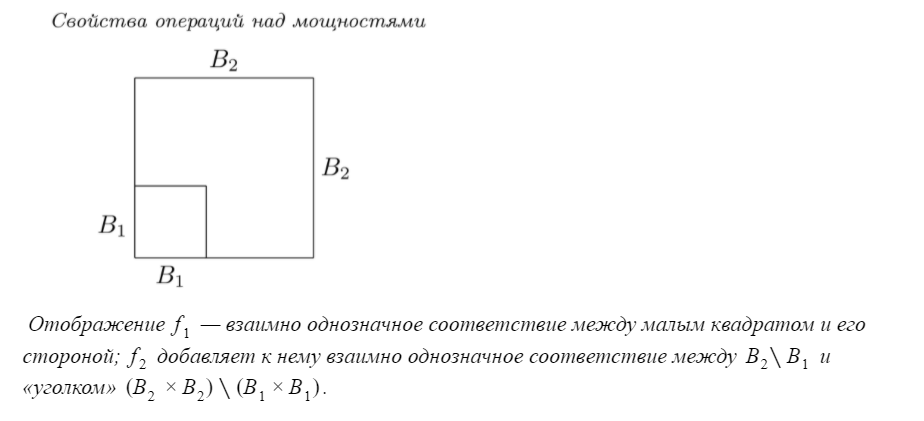
\includegraphics[width=14cm]{images/2.12 1.png}
\end{center}

Теперь применим лемму Цорна. Для этого нужно убедиться, что любое линейно упорядоченное (в смысле описанного порядка) множество пар указанного вида имеет верхнюю границу. В самом деле, объединим все первые компоненты этих пар; пусть $B$ — их объединение. Как обычно, согласованность отображений (гарантируемая определением порядка) позволяет соединить отображения в одно. Это отображение (назовём его $f$) отображает $B$ в $B \times B$. Оно будет инъекцией: значения $f(b')$ и $f(b'')$ при различных $b'$ и $b''$ различны (возьмем большее из множеств, которым принадлежат $b'$ и $b''$; на нём $f$ является инъекцией по предположению). С другой стороны, $f$ является сюръекцией: для любой пары $(b', b'') \in B \times B$ возьмём множества, из которых произошли $b'$ и $b''$, выберем из них большее и вспомним, что мы имели взаимно однозначное соответствие между ним и его квадратом.

По лемме Цорна в нашем частично упорядоченном множестве существует максимальный элемент. Пусть этот элемент есть $(B, f)$. Мы знаем, что $f$ есть взаимно однозначное соответствие между $B$ и $B \times B$ и потому $|B| = |B| \times |B|$. Теперь есть две возможности. Если $B$ равномощно $A$, то $B \times B$ равномощно $A \times A$ и всё доказано. Осталось рассмотреть случай, когда $B$ не равномощно $A$, то есть имеет меньшую мощность (большей оно иметь не может, будучи подмножеством). Пусть $C$ -- оставшаяся часть $A$, то есть $A \backslash B$.

Тогда $|A| = |B| + |C| = max(|B|, |C|)$, следовательно, $C$ равномощно $A$ и больше $B$ по мощности. Возьмём в $C$ часть $C'$, равномощную $B$, и положим $B' = B + C'$.

\begin{center}
    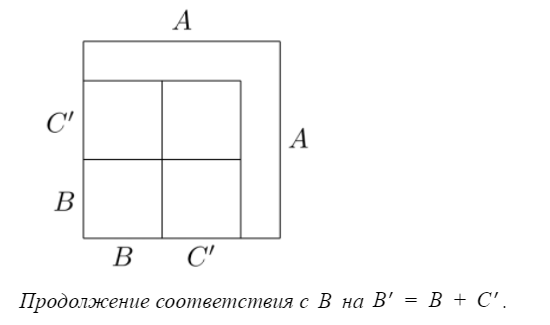
\includegraphics[width=7.5cm]{images/2.12 2.png}
\end{center}

Обе части множества $B'$ равномощны $B$. Поэтому $B' \times B'$ разбивается на $4$ части, каждая из которых равномощна $B \times B$, и, следовательно, равномощна B (т.к. $C', (B' \times B'), (B \times B)$  равномощны $B$). В итоге мы получаем большую пару $(B', f')$, что противоречит утверждению леммы Цорна о максимальности. Таким образом, этот случай невозможен.